
\section{Ranking SEO}
\subsubsection{Ranking e SEO}
Oltre ai classici fattori interni che influenzano il posizionamento, altre pratiche SEO adottate per migliorare il posizionamento del sito web nei motori di ricerca includono:
\begin{itemize}
    \item \textbf{Microformati nel footer:} utilizzo di microformati per le informazioni di contatto. Sono stati inseriti selettori di attributo \texttt{class} riconosciuti dai motori di ricerca per evidenziare il contenuto in modo semanticamente corretto. Il tag \texttt{address} da solo non è sufficiente poiché non specifica la natura delle informazioni contenute. È stato inserito anche Aggiunto anche \textit{rel="e"} per la pagina social;
    \item \textbf{Aggiunta di call to action nelle meta description:} le descrizioni delle pagine contengono inviti all'azione per incoraggiare gli utenti a visitare il sito web (es. "Trova subito il match per te!");
\end{itemize}
\paragraph{Peso delle pagine}
Durante lo sviluppo del progetto abbiamo notato che le pagine che mostrano molte immagini risultavano molto pesanti da renderizzare. Abbiamo modificato la funzione che importa le immagini per comprimere le immagini arrivano ai 40KB prima di inserirle nel server. Le immagini perdono un po' di qualità ma migliorano notevolmente i tempi di caricamento delle pagine.\\
Inoltre in alcune pagine con le schede a tabs (come quelle che mostrano un layout a schede nell'area amministatore) abbiamo sfruttato il \texttt{display:none} di css per nascondere il contenuto della scheda non attiva. In questo modo, il browser non scarica i dati ad ogni cambio di scheda, ma tutti in una singola volta al caricamento iniziale della pagina. \\
Questa scelta migliora l'esperienza utente, riducendo i tempi di attesa durante la navigazione tra le schede.
\subsubsection*{Lighthouse}
Per valutare le prestazioni abbiamo utilizzato lo strumento Lighthouse integrato in Chrome DevTools.\\ I risultati mostrano ottime prestazioni. Qui di seguito sono riportati gli screenshot dei risultati delle pagine più critiche:
\begin{figure}[H]
    \centering
    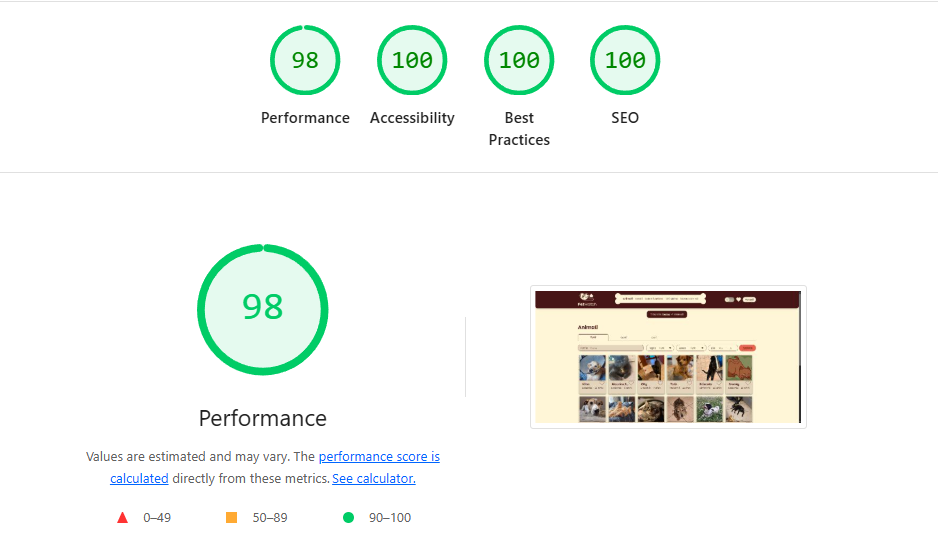
\includegraphics[width=0.8\textwidth]{assets/lighthouse-animali.png}
    \caption{Risultati Lighthouse per la pagina animali}
\end{figure}
\begin{figure}[H]
    \centering
    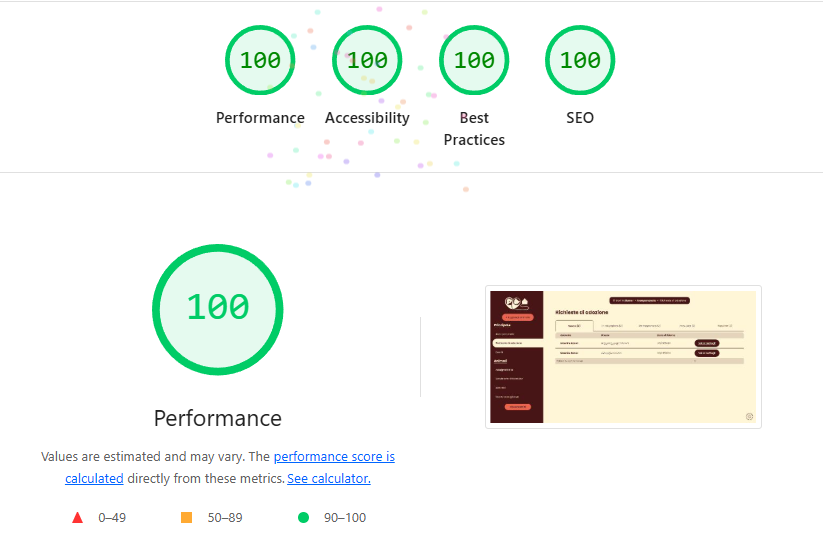
\includegraphics[width=0.8\textwidth]{assets/lighthouse-admin.png}
    \caption{Risultati Lighthouse per la pagina area personale}
\end{figure}
% BROOOOOOOÒ LA ROBA DELLE TABS